%----------------------------------------------------------------------------
\chapter{\LaTeX-eszközök}
\label{sec:LatexTools}
%----------------------------------------------------------------------------
\section{A szerkesztéshez használatos eszközök}
%----------------------------------------------------------------------------
Ez a sablon TeXstudio 2.8.8 szerkesztővel készült. A TeXstudio egy platformfüggetlen, Windows, Linux és Mac OS alatt is elérhető \LaTeX-szerkesztőprogram számtalan hasznos szolgáltatással (\refstruc{fig:TeXstudio}). A szoftver ingyenesen letölthető\footnote{A TeXstudio hivatalos oldala: \url{http://texstudio.sourceforge.net/}}.

\begin{figure}[!ht]
\centering
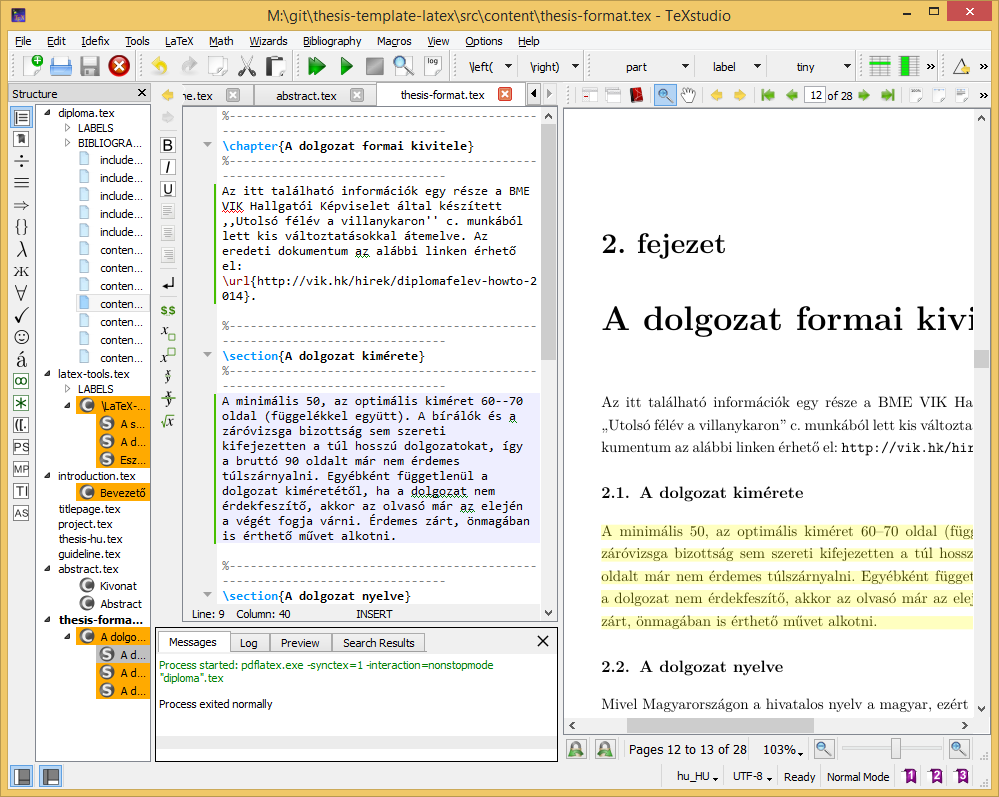
\includegraphics[width=150mm, keepaspectratio]{figures/TeXstudio.png}
\caption{A TeXstudio \LaTeX-szerkesztő.}
\label{fig:TeXstudio}
\end{figure}

A TeXstudio telepítése után érdemes még letölteni a magyar nyelvű helyesírásellenőrző-szótárakat hozzá. A TeXstudio az OpenOffice-hoz használatos formátumot tudja kezelni. A TeXstudio beállításainál a \verb+General+ fülön a \verb+Dictionaries+ résznél tudjuk megadni, hogy melyik szótárat használja.

Egy másik használható Windows alapú szerkesztőprogram a LEd\footnote{A LEd hivatalos oldala: \url{http://www.latexeditor.org/}} (LaTeX Editor), a TeXstudio azonban stabilabb, gyorsabb, és jobban használható.

%----------------------------------------------------------------------------
\section{A dokumentum lefordítása Windows alatt}
%----------------------------------------------------------------------------
A TeXstudio és a LEd kizárólag szerkesztőprogram (bár az utóbbiban DVI-nézegető is van), így a dokumentum fordításához szükséges eszközöket nem tartalmazza. Windows alatt alapvetően két lehetőség közül érdemes választani: MiKTeX (\url{http://miktex.org/}) és TeX Live (\url{http://www.tug.org/texlive/}) programcsomag. Az utóbbi működik Mac OS X, GNU/Linux alatt és Unix-származékokon is. A MiKTeX egy alapcsomag telepítése után mindig letölti a használt funkciókhoz szükséges, de lokálisan hiányzó \TeX-csomagokat, míg a TeX Live DVD ISO verzóban férhető hozzá. Ez a dokumentum TeX Live 2008 programcsomag segítségével fordult, amelynek DVD ISO verziója a megadott oldalról letölthető. A sablon lefordításához a disztribúcióban szereplő \verb+magyar.ldf+ fájlt a \verb+http://www.math.bme.hu/latex/+ változatra kell cserélni, vagy az utóbbi változatot be kell másolni a projekt-könyvtárba (ahogy ezt meg is tettük a sablonban) különben anomáliák tapasztalhatók a dokumentumban (pl. az ábra- és táblázat-aláírások formátuma nem a beállított lesz, vagy bizonyos oldalakon megjelenik alapértelmezésben egy fejléc). A TeX Live 2008-at még nem kell külön telepíteni a gépre, elegendő DVD-ről (vagy az ISO fájlból közvetlenül, pl. DaemonTools-szal) használni.

Ha a MiKTeX csomagot használjuk, akkor parancssorból a következő módon tudjuk újrafordítani a teljes dokumentumot:

\begin{lstlisting}[language=bash,frame=single,float=!ht]
$ texify -p thesis.tex
\end{lstlisting}

A \verb+texify+ parancs a MiKTex programcsomag \verb+miktex/bin+ alkönyvtárában található. A parancs gondoskodik arról, hogy a szükséges lépéseket (fordítás, hivatkozások generálása stb.) a megfelelő sorrendben elvégezze. A \verb+-p+ kapcsoló hatására PDF-et generál. A fordítást és az ideiglenes fájlok törlését elvégezhetjük a sablonhoz mellékelt \verb+manual_build.bat+ szkript segítségével is.

A \TeX-eszközöket tartalmazó programcsomag binárisainak elérési útját gyakran be kell állítani a szerkesztőprogramban, például TeXstudio esetén legegyszerűbben az \verb+Options / Configure TeXstudio... / Commands+ menüponttal előhívott dialógusablakban tehetjük ezt meg.

A PDF-\LaTeX~használata esetén a generált dokumentum közvetlenül PDF-formátumban áll rendelkezésre. Amennyiben a PDF-fájl egy PDF-nézőben (pl. Adobe Acrobat Reader vagy Foxit PDF Reader) meg van nyitva, akkor a fájlleírót a PDF-néző program tipikusan lefoglalja. Ilyen esetben a dokumentum újrafordítása hibaüzenettel kilép. Ha bezárjuk és újra megnyitjuk a PDF dokumentumot, akkor pedig a PDF-nézők többsége az első oldalon nyitja meg a dokumentumot, nem a legutóbb olvasott oldalon. Ezzel szemben például az egyszerű és ingyenes \textcolor{blue}{Sumatra PDF} nevű program képes arra, hogy a megnyitott dokumentum megváltozását detektálja, és frissítse a nézetet az aktuális oldal megtartásával.

%----------------------------------------------------------------------------
\section{Eszközök Linuxhoz}
%----------------------------------------------------------------------------
Linux operációs rendszer alatt is rengeteg szerkesztőprogram van, pl. a KDE alapú Kile jól használható. Ez ingyenesen letölthető, vagy éppenséggel az adott Linux-disztribúció eleve tartalmazza, ahogyan a dokumentum fordításához szükséges csomagokat is. Az Ubuntu Linux disztribúciók alatt például legtöbbször a \verb+texlive-*+ csomagok telepítésével használhatók a \LaTeX-eszközök. A jelen sablon fordításához szükséges csomagok (kb. 0,5 GB) az alábbi paranccsal telepíthetők:

\begin{lstlisting}[language=bash,morekeywords={sudo,apt\-get},alsoletter={-},breaklines=true]
$ sudo apt-get install texlive-latex-extra texlive-fonts-extra texlive-fonts-recommended texlive-xetex texlive-science
\end{lstlisting}

Amennyiben egy újabb csomag hozzáadása után hiányzó fájlra utaló hibát kapunk a fordítótól, telepítenünk kell az azt tartalmazó TeX Live csomagot. Ha pl. a \verb+bibentry+ csomagot szeretnénk használni, futtassuk az alábbi parancsot:

\begin{lstlisting}[language=bash,morekeywords={apt\-cache},alsoletter={-},breaklines=true]
$ apt-cache search bibentry
texlive-luatex - TeX Live: LuaTeX packages
\end{lstlisting}

Majd telepítsük fel a megfelelő TeX Live csomagot, jelen esetben a `texlive-lualatex`-et. (Egy LaTeX csomag több TeX Live csomagban is szerepelhet.)

Ha gyakran szerkesztünk más \LaTeX dokumentumokat is, kényelmes és biztos megoldás a teljes TeX Live disztribúció telepítése, ez azonban kb. 4 GB helyet igényel.

\begin{lstlisting}[language=bash,morekeywords={sudo,apt\-get},alsoletter={-},breaklines=true]
sudo apt-get install texlive-full
\end{lstlisting}
